\section{Implementation}\label{sec:implementation}
We use Blender to render a scene consisting of a model of a monkey's head, a
mirror, five light sources, and a camera. The monkey's head is perfectly
Lambertian and the mirror perfectly reflective. The light sources are
positioned at various angles above the monkey's head and are perfectly
directional, which means that the flux of the light does not depend on
position. (This is a frequent approximation of an infinitely distant point
source or of light from the Sun.) For convenience, the camera is positioned
exactly in front of the monkey's head facing it at a position such that the
entire head and none of the mirror surface is in frame. In each image, exactly
one of the five light sources is turned on. See Figure~\ref{fig:blender-scene}
for reference.

Five images are rendered, one for each light source, with the mirror in the
scene. Five more such images are rendered with the mirror removed as a baseline
using the original (mirrorless) photometric stereo algorithm. In addition, the
96 \texttt{catPNG} images from the DiLiGenT dataset~\cite{shi} are used to
verify the photometric stereo implementation against a known ground truth.

Between three and five frames are used for computing all possible normals at
each pixel for the mirrored dataset. As discussed in
Section~\ref{sec:technical}, this results in $3^3$ to $3^5$ candidates at each
pixel, and the main task is to choose the ``correct'' one, which corresponds to
the correct labelling of the combination of lights that illuminated it. (The
full 96 images are used for computing normals on \texttt{catPNG}, but there is
no mirror involved and therefore only one possible normal at each pixel.) Three
approaches to pixel labelling are explored.
\begin{figure}
  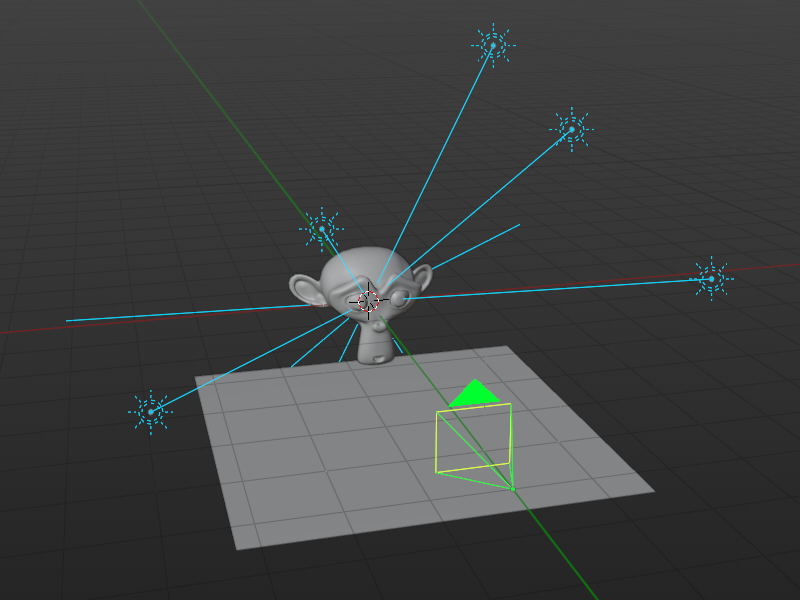
\includegraphics[width=0.5\columnwidth]{images/blender-scene_1.png}
  \nolinebreak
  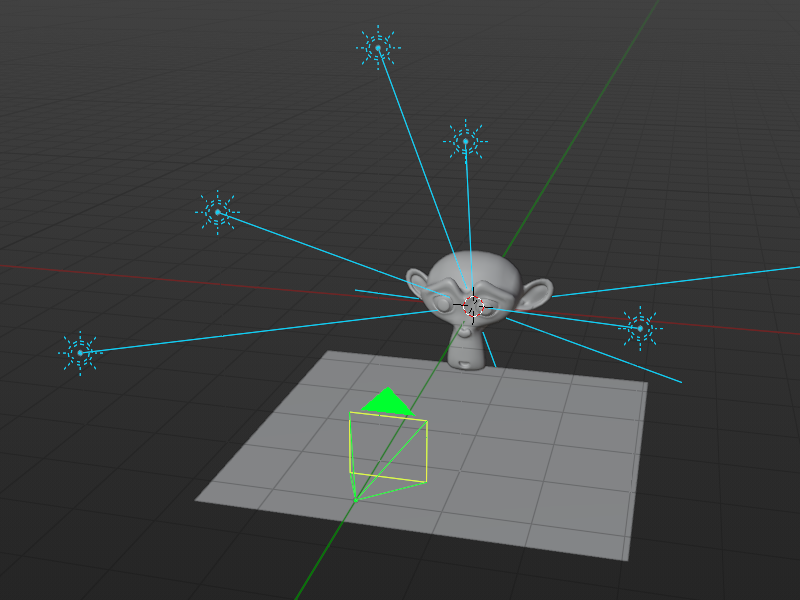
\includegraphics[width=0.5\columnwidth]{images/blender-scene_2.png}
  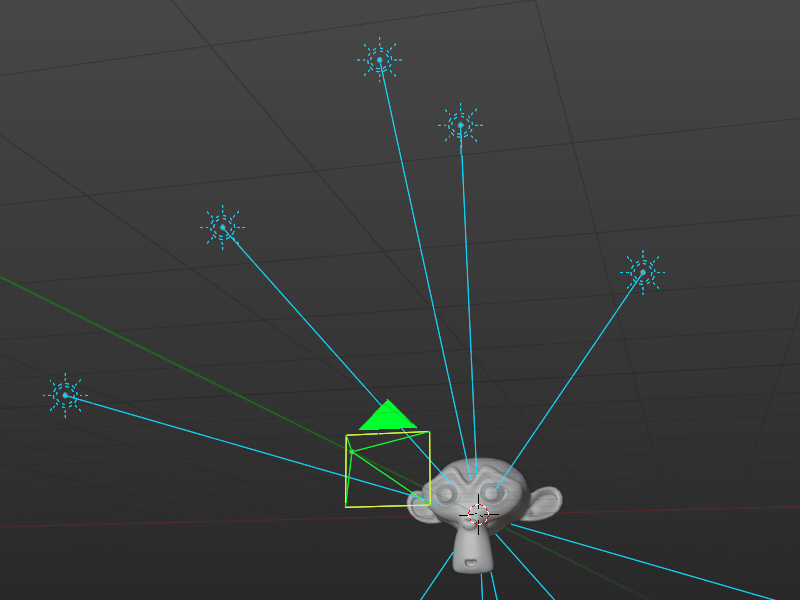
\includegraphics[width=0.5\columnwidth]{images/blender-scene_3.png}
  \nolinebreak
  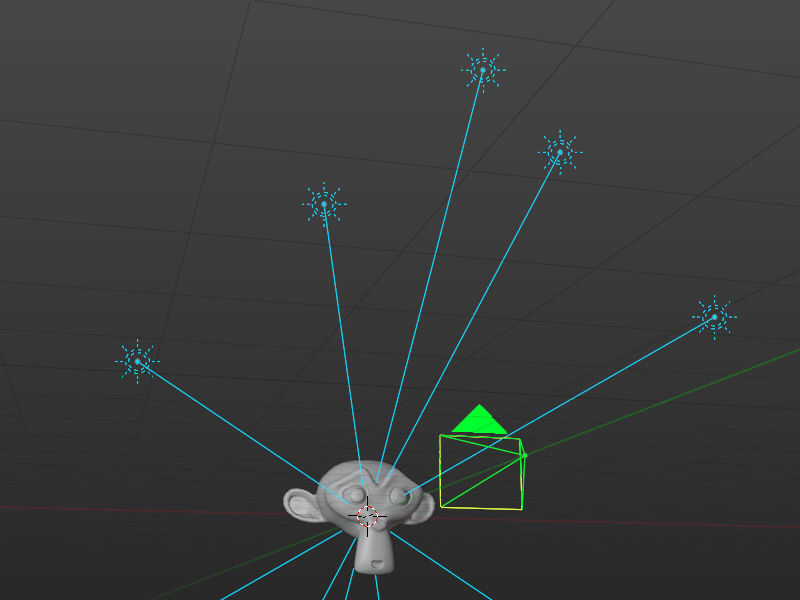
\includegraphics[width=0.5\columnwidth]{images/blender-scene_4.png}
  \caption{Four views of the scene in Blender used to render image data. Note
  that the positions of the light sources along their rays do not matter as
  they are purely directional.}\label{fig:blender-scene}
\end{figure}
\subsection{Least-Squares Approach}\label{sec:least-squares}
For each pixel location, we attempt to reconstruct the pixel according to
\begin{equation}
  \pixel_{i k} = \tilde{\light}_{i k} \point_k
\end{equation}
for each candidate $1 \le k \le 3^N$ and choose the one with the lowest squared
error
\begin{equation}
  \mathrm{error} = \sum_{i = 1}^N {\left(\pixel_i - \pixel_{i k}\right)}^2
\end{equation}
Note that this approach is only possible for $N \ge 4$. For $N = 3$, the
pseudoinverse in Equation~\ref{eq:pseudoinverse} is simply the inverse of
$\lights$ and the squared error is always zero.
\subsection{Forest-Building Approach}
By assumping the normal $\hat{\point} = \frac{\point}{\|\point\|}$ varies
smoothly across large regions of the object (its faces), we associate
candidates of $\point_k(x, y)$ with likely candidates $\point_k(x \pm 1, y)$
and $\point_k(x, y \pm 1)$ of its neighbors. We do using a variant on
breadth-first search: while processing $\point_k(x, y)$, we mark as its
neighbor the $\point_{k'}(x + 1, y)$ for
\begin{equation}
  \arg\max_{1 \le k' \le 3^N} \frac{\point_k(x, y) \cdot \point_{k'}(x + 1, y)}{\|\point_k(x, y)\| \, \|\point_{k'}(x + 1, y)\|}
\end{equation}
(the cosine similarity) and similarly with $\point_{k'}(x - 1, y)$,
$\point_{k'}(x, y + 1)$, and $\point_{k'}(x, y - 1)$. This forms a forest whose
connected components correspond to faces of the object. For a given pixel
position $(x, y)$, we take the candidate $\point$ that belongs to the largest
connected component.

This approach was only seriously considered due to an error in calculating its
complexity, which turns out to be $O \left({\left(3^n\right)}^3\right)$. As it
became clear that it was terribly impractical, this approach was abandoned.
\subsection{Energy-Minimizing Approach}
Instead of performing the costly forest construction described above, we could
pose the labelling task as an energy-minimization problem as described
in~\cite{schechner}. The objective function combines a data term to minimize
reconstruction error of $I_{i k}$ (as in Section~\ref{sec:least-squares}) as
well as a smoothness term that penalizes the difference in \emph{label} (that
is, the combination of sources visible to a pixel) rather than the difference
in the normal vector itself. Schechner et al.~\cite{schechner} propose a
graph-cut-based approximation to this otherwise NP-complete problem and
demonstrate that it is a reliable approach to light combination labelling for
photometric stereo with two or more lights per frame, which is exactly how we
characterize our mirrored problem.

